%!TEX root = ../report.tex
\chapter{Experiments and results}
\label{cha:Experiments}
In this chapter the planning, setup, and results from experiments are presented. The results use time and accuracy as metrics, and is used to evaluate how different traversal criteria, and datasets affect a search.

\section{Experimental plan}
\label{sec:experimentalPlan}
The goal of the experiments is to gather data for comparison of data types searched and criteria for vertices to follow. When comparing, speed and accuracy will be the metrics used. In total, nine different searches will be conducted, one using spatial data for input and roots, one using temporal data for input and roots, and one combining the two, using spatiotemporal data for input and roots. For each of these vertex types, there will also be different criteria for how the graph will be explored. The first method follows all predicates, excluding connections to types and classes, and will have a max distance of two. The second method follows the same predicates as the first but has the max distance set to one. Finally, a criterion for following only predicates from vertices with at least one keyword match is used.

When comparing the methods, the goal is to see how reducing the amount of data search will affect speed and accuracy of the search, and how differences in distance and edges followed differs based on the starting data.

\subsection{Time}
When timing the algorithm, two different times is measured, time for each search, and time used for traversing and ranking a single root. In addition to these, avg. vertices visited for each root will also be used. Taking the average of these over a large input set should generate an appropriate result. Both time metrics measure how fast results are found, so the results should be similar if the input data does not contain a high number of highly connected vertices.

The timing of the algorithm should be the same as any breath first search, $\Theta(\mathsf{V} + \mathsf{E})$ so that the best case is visiting only the first vertex, and the worst case is traversing the entire graph.

\subsection{Scoring and ranking}
Each subgraph is given a score. This score will be used to see how pruning, and difference in predicates can lead to differences in the result tree. Two metrics for accuracy will be used, avg. accuracy for each result and avg. highest accuracy for each query.

\section{Experimental setup}
\label{sec:experimentalSetup}
All experiments was run on a single laptop with the specifications listed in table \ref{table:laptop}. The code is written in Java, using openJDK 11.0.7 and building with Gradle 6.0. For triple store, Jena tdb storage was used, using version 3.14.0 of Jena.
\begin{table}[h]
    \centering
    \begin{tabular}{ll}
        \hline
        OS     & Ubuntu 19.10 x86\_64              \\
        Host   & 20KGS0N400 ThinkPad X1 Carbon 6th \\
        Kernel & 5.3.0-46-generic                  \\
        CPU    & Intel i5-8350U (8) @ 3.600GHz     \\
        Memory & 15760MiB                          \\
        \hline
    \end{tabular}
    \caption{Platform used for experiments}
    \label{table:laptop}
\end{table}

\subsection{Data set}
All of the data used is from YAGO. YAGO was selected for the large open data set, rich taxonomy, and for the spatial and temporal parts of the ontology. There are several data sets available for download, divided into categories. For running experiments data from taxonomy, core, and GeoNames were selected. From the taxonomy category, all data sets where used. This data describes class structure, entities, and defines relationships.

From the core category all data was also used. The core contains most of the data used in the graph. This includes dates, relationships between nodes, literals, and labels. Most of the vertices and edges used in the experiment comes from this category, but this data can be further structured using some of the data from other categories.

GeoNames contains data and structure for geographical vertices. These vertices have a hierarchical structure based on places being located within other places. In addition, the data contains literals for coordinates, alternative names and links for neighbors. In addition, the category contains additional classes and types specific for the geographical vertices.

Before the data could be loaded into a store, some preprocessing was necessary. This includes replacing non-Unicode character, and replacing spaces with underscore in URIs. In addition, the data from YAGO contained some illegal characters for Jena, such as double quoted URIs and illegal escape sequences. There were also some unterminated TTL lines. All the data was run through a sed script to ensure correctly formatted data for Jena. After formatting the data correctly, a persistent TDB storage was created using TDBloader from Jena.
% sed -i 's/|/-/g' ./* && sed -i 's/\\\\/-/g' ./* && sed -i 's/–/-/g' ./*

\subsection{Queries}
When selecting words for the queries, all nodes in the graph was scanned to count word frequency. This list was sorted based on number of occurrences, stop words and numbers were removed. From this shortened list, the top 150 words were chosen, based on vocabulary size needed to meet more than half of nodes \cite{zipf,worthington1996using}. From this list of 150 words, a final set of 10 words was chosen at random. It is worth noting that all words are from the name of a vertex, so the list of words does not reflect natural language.

When selecting places, a set of 7 places were manually chosen. This choice was made to ensure places from different parts of the world, and difference in population and language. With these differences, root vertices found should have variation in edges, differences in keyword vertices discovered, and paths discovered for shared keyword vertices.

Date selection for temporal search was done manually. This selection included a combination of non-significant dates, and significant dates. The selection was made to have a high probability of finding hits and ensure that the vertices have variation in the amount of edges.

\subsection{Combining data and queries}
When running the experiments, the same set of query words was used for all runs. For each type of data, spatial, temporal, and spatiotemporal, the query words were combined in five groups containing two words, and four groups containing four words. Variation in the amount of words used would affect both the chance of hitting keyword vertices, and the score of the trees discovered.

\subsection{Max. distance and following edges}
For each of the data types a total of three different exploration methods was used. One with a max. distance of 1 from the root node, one with a max. distance of 2, and one where only edges leading to a keyword vertex would be explored further. Using a max. depth of 2 would serve as a base line for the comparison. The two other methods were used to see how much distance from the root would affect the accuracy, and if optimal graphs could be found even with a severe limitation put on the search.

\section{Experimental results}
\label{sec:experimentalResults}
\subsection{Code profiling and external impact}
Because the platform used to run the experiments was a laptop, there are external factors that affect the result. One such factor is the CPU of the laptop overheating and throttling, meaning it does not run at top speed, and instead moves between a high and low speed in intervals. This can clearly be seen in figure \ref{fig:profile2}, where the CPU throttles between $\approx$20\% and $\approx$32\% with the high value lasting for about 20 seconds, and the lower values for just under a minute. The figure displays three runs of the algorithm, the first two being warmup runs, and the third is a profile run. During the initiation of each run there is a spike in CPU usage almost reaching 70\%. CPU usage is also split in to two categories, where blue is system load, and green is process load. During the warmup, the process load is low, and is slightly increased during the profiling.

Memory usage and garbage collection will also affect the performance. In figure \ref{fig:profile1} and \ref{fig:profileFollow} the memory usage is low, and there is less garbage collection. Compare this to the runs with a distance of two, where garbage collection is done often. It is also worth noting that the algorithm runs on two threads, with a further four used for IO. Most IO operations are from reading vertices from the triple store.

\begin{figure}[hb]
	\centering
	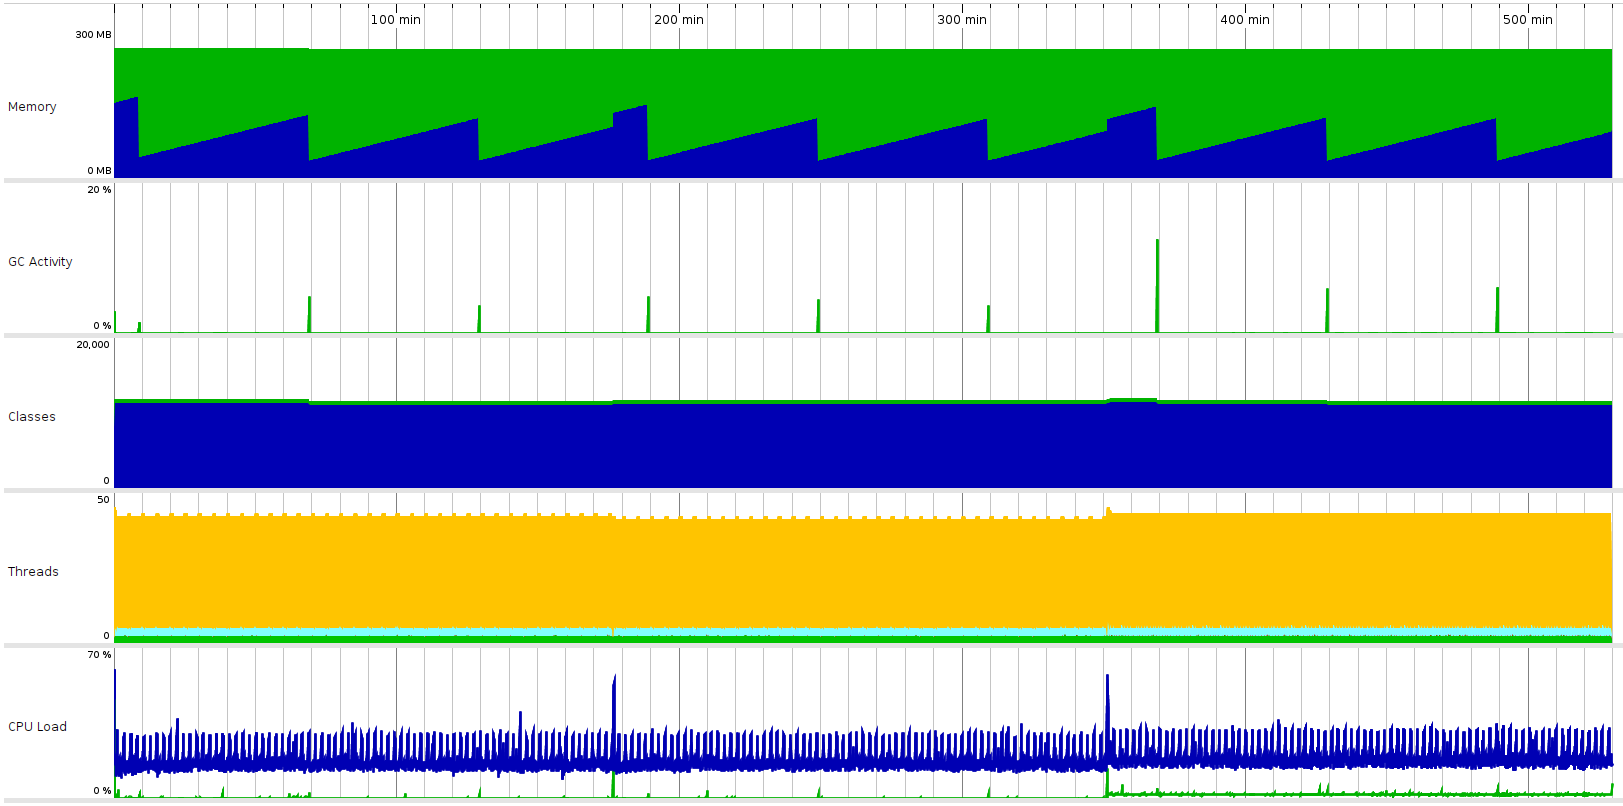
\includegraphics[scale=0.25]{figs/profile2.png}
	\caption{Code profile of spatial data using distance 2.}
	\label{fig:profile2}
\end{figure}
 
\begin{figure}
	\centering
	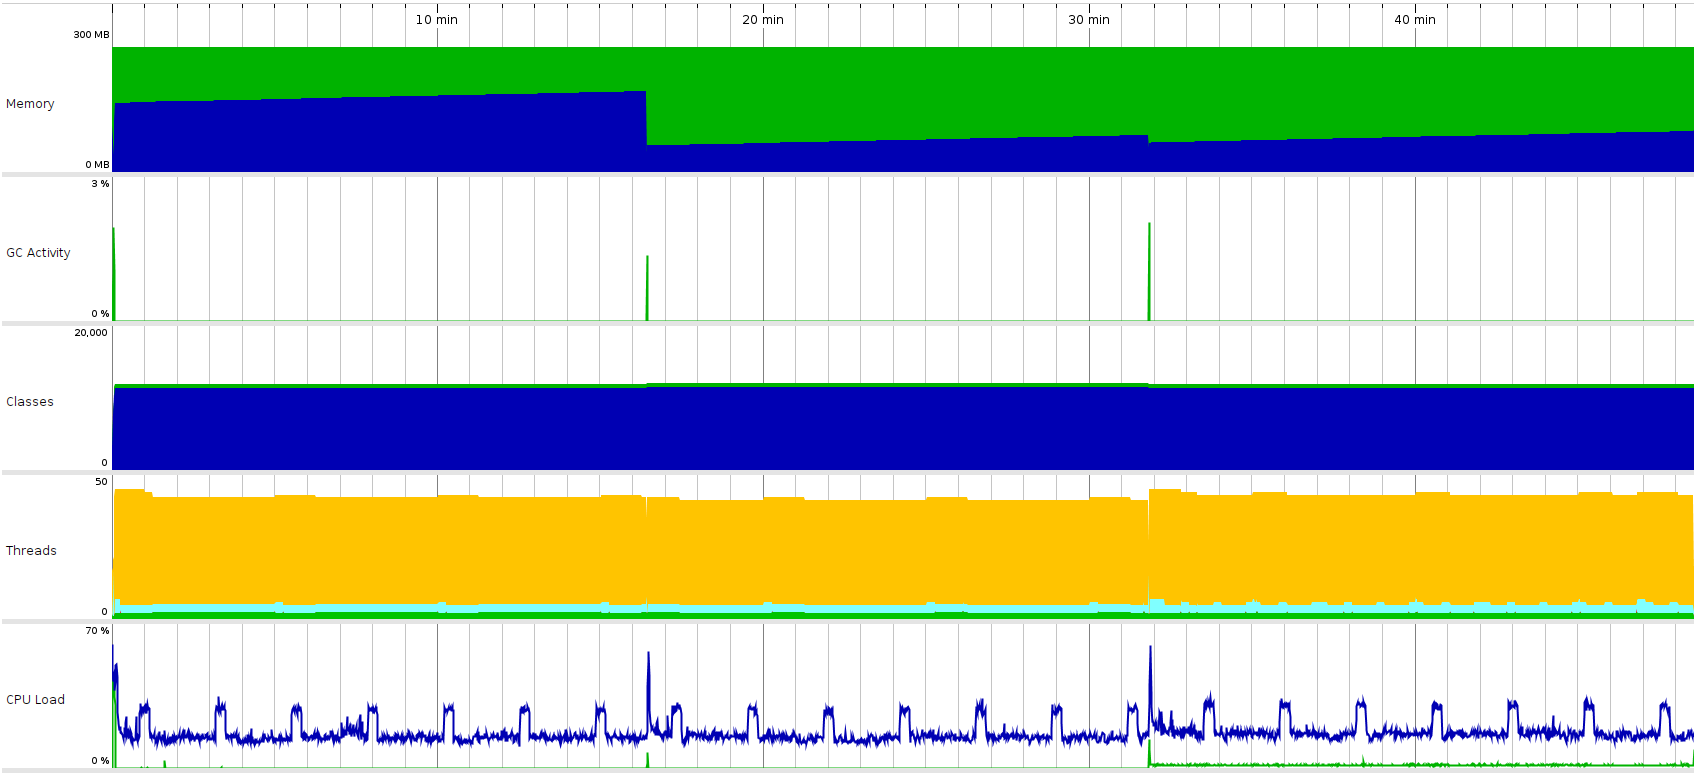
\includegraphics[scale=0.245]{figs/profile1.png}
	\caption{Code profile spatial data and distance 1}
	\label{fig:profile1}
\end{figure}
%
\begin{figure}
	\centering
	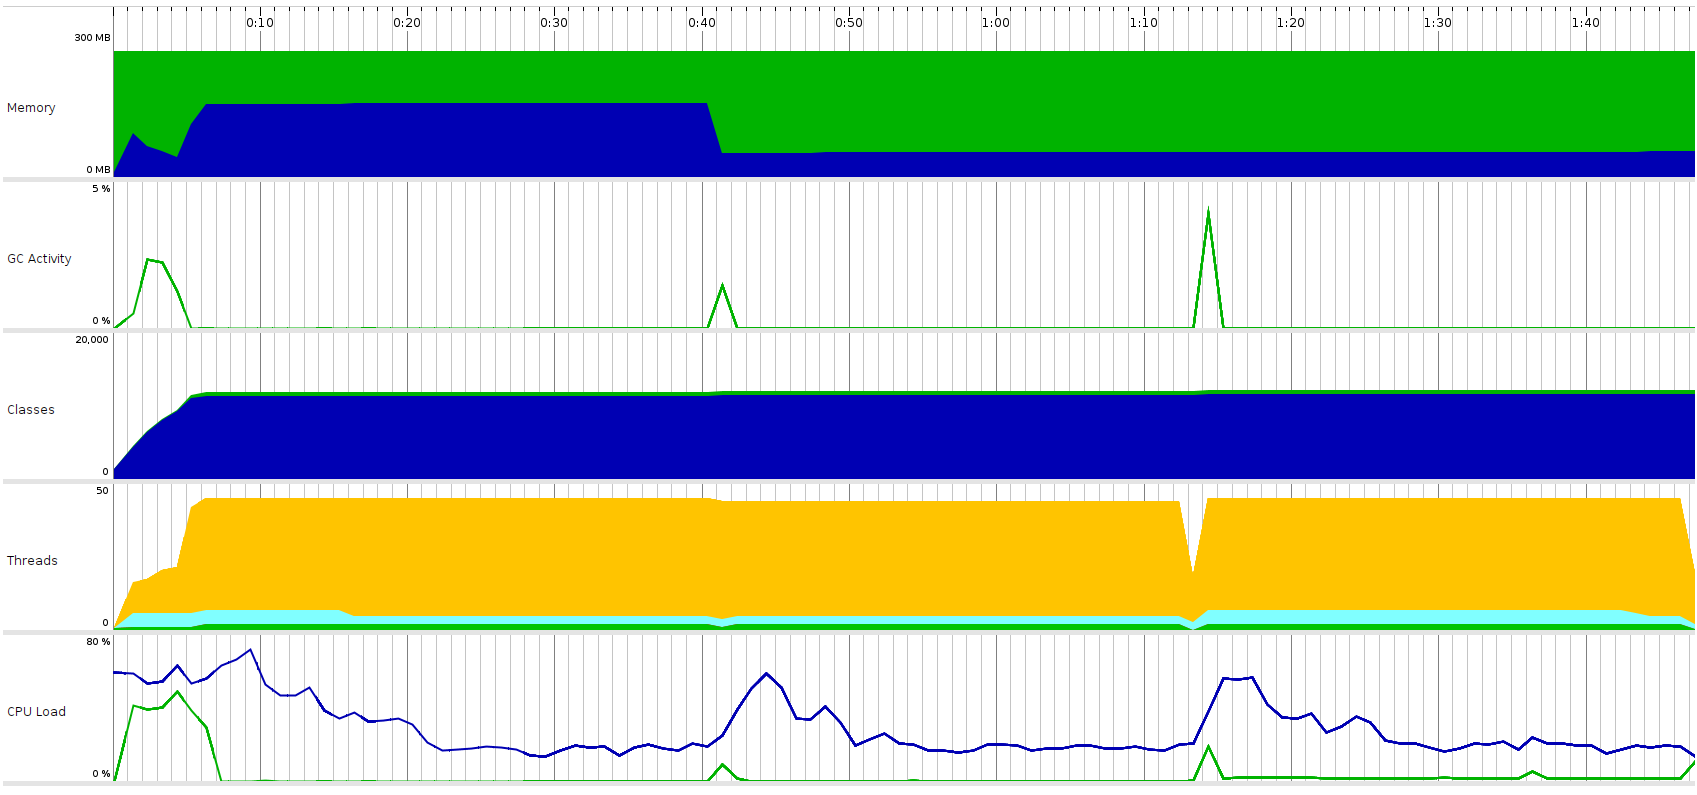
\includegraphics[scale=0.245]{figs/profileHits.png}
	\caption{Code profile of spatial data following vertices with hits}
	\label{fig:profileFollow}
\end{figure}
\FloatBarrier

\subsection{Effect of distance from root}
When traversing a graph, the number of vertices visited will heavily impact the time used. When the max. distance of the search increase, the number of vertices visited will grow with the number of roots discovered times the distance from the root. Looking at table \ref{table:followAll2} we see that the amount of roots found for a query is the most significant factor for the speed and amount of vertices visited. Since there only is three data points, no broad conclusion can be drawn, but in figure \ref{fig:linReg1and2} a trend can be seen, and all points line up well. This indicates a linear increase of vertices visited, where the slope is based on the amount of edges the vertices have and the depth from the root vertex. Comparing this to the more detailed graph \ref{fig:linregQueries} we can see that the time used for a query still follows a linear increase. Using a distance of 2, the time varies more than the other two methods, but the timings appear to increase linearly based on the number of roots discovered. In graph \ref{fig:linregQueries} all the different data types are added, and since both temporal, and spatiotemporal queries have fewer roots per query, most of the data points are clustered in the lower end of the graph. All three data sets contain one point for each query with at least one root, totaling 388 points for each traversal method.

From the results it is clear that increasing the distance traveled from the root have the most significant impact on both speed and accuracy. When the distance is increased many more vertices are visited, so that the chance of finding a keyword match is increased. Visiting more vertices will also take significantly more time. From figure \ref{fig:linregQueries} it is also clear that the amount of roots discovered for a query will make a significant difference. This difference is further amplified when the distance is higher. Even though the increase in time is linear, the slope is much steeper for traversals with higher distance, resulting in significant time increases.

\begin{table}[h]
	\caption{Follow all edges, max. distance 2}
	\label{table:followAll2}
	\begin{tabular}{ |p{3cm}||p{3cm}|p{3cm}|p{3cm}|  }
		\hline
		\multicolumn{4}{|c|}{Traversal following all edges max. distance 2}                         \\
		\hline
		Result type                    & Temporal data  & Spatial data  & Spatial and temporal data	\\
		\hline
		Avg. time per query (ms)       & 27\,679        & 166\,479      & 1\,842                    \\
		Avg. roots per query           & 192            & 1\,527        & 10                        \\
		Avg. nodes per root            & 3\,097         & 3\,684        & 4\,843                    \\
		Avg. nodes visited per query   & 594\,683       & 5\,626\,989   & 49\,719                   \\
		Avg. accuracy per result       & 0.075          & 0.077         & 0.066                     \\
		Avg. top accuracy per query    & 0.231          & 0.280         & 0.108                     \\
		Query miss (no keywords found) & 24/63 (38.1\%) & 6/63 (10.5\%) & 357/441 (81.0\%)          \\
		\hline
	\end{tabular}
\end{table}

\begin{figure}
	\centering
	\begin{tikzpicture}
	\pgfplotsset{width=10cm,
		compat=1.3,
		legend style={font=\footnotesize}}
	\begin{axis}[
			xlabel={Avg. roots per query},
			ylabel={Time in ms.},
			legend cell align=left,
			legend pos=north west]
		\addplot[only marks] table[row sep=\\]{
				X Y\\
				192 27679\\
				1527 166479\\
				10 1842\\
			};
		\addlegendentry{Max. distance 2}
		\addplot[only marks] table[row sep=\\]{
				X Y\\
				192 4111\\
				1527 14618\\
				10 467\\
			};
		\addlegendentry{Max. distance 1}
		\addplot table[row sep=\\,
				y={create col/linear regression={y=Y}}] % compute a linear regression from the
			%input table
			{
				X Y\\
				192 27679\\
				1527 166479\\
				10 1842\\
			};
			\addlegendentry{%
			$\pgfmathprintnumber{\pgfplotstableregressiona} \cdot x
				\pgfmathprintnumber[print sign]{\pgfplotstableregressionb}$ lin. Regression} %
		\addplot table[row sep=\\,
				y={create col/linear regression={y=Y}}] % compute a linear regression from the
			%input table
			{
				X Y\\
				192 4111\\
				1527 14618\\
				10 467\\
			};
		\addlegendentry{%
			$\pgfmathprintnumber{\pgfplotstableregressiona} \cdot x
				\pgfmathprintnumber[print sign]{\pgfplotstableregressionb}$ lin. Regression} %
	\end{axis}
\end{tikzpicture}
	\caption{Linear regression for time and roots}
	\label{fig:linReg1and2}
\end{figure}
 
\begin{figure}
	\centering
	\begin{tikzpicture}
	\pgfplotsset{width=\textwidth,
		compat=1.3,
		legend style={font=\footnotesize}}
	\begin{axis}[
			xlabel={Total roots found},
			ylabel={Time in ms.},
			legend cell align=left,
			legend pos=north west]
		\pgfplotstableread{graphTab/dist2Data.ssv}\distTwo;
		\pgfplotstableread{graphTab/dist1Data.ssv}\distOne;
		\pgfplotstableread{graphTab/followHits.ssv}\follow;

		\addplot[black, only marks] table[row sep=\\]{\distTwo};
		\addlegendentry{Max. distance 2}
		\addplot[blue, only marks] table[row sep=\\]{\distOne};
		\addlegendentry{Max. distance 1}
		\addplot[red, only marks] table[row sep=\\]{\follow};
		\addlegendentry{Follow all hits}

		\addplot table[row sep=\\,
				y={create col/linear regression={y=Y}}] {\distTwo};
		\xdef\slopeA{\pgfplotstableregressiona}
		\xdef\interceptA{\pgfplotstableregressionb}
		\addlegendentry{%
			$\pgfmathprintnumber{\slopeA} \cdot x
				\pgfmathprintnumber[print sign]{\interceptA}$ lin. Regression} %

		\addplot table[row sep=\\,
				y={create col/linear regression={y=Y}}] {\distOne};
		\xdef\slopeB{\pgfplotstableregressiona}
		\xdef\interceptB{\pgfplotstableregressionb}
		\addlegendentry{%
			$\pgfmathprintnumber{\slopeB} \cdot x
				\pgfmathprintnumber[print sign]{\interceptB}$ lin. Regression} %

		\addplot table[row sep=\\,
				y={create col/linear regression={y=Y}}] {\follow};
		\xdef\slopeC{\pgfplotstableregressiona}
		\xdef\interceptC{\pgfplotstableregressionb}
		\addlegendentry{%
			$\pgfmathprintnumber{\slopeC} \cdot x
				\pgfmathprintnumber[print sign]{\interceptC}$ lin. Regression} %
	\end{axis}
\end{tikzpicture}
	\caption{Linear regression for time and roots}
	\label{fig:linregQueries}
\end{figure}

\subsection{Effect of following specific edges}
In table \ref{table:followHits} we see that very few vertices with a keyword are directly connected to other vertices with a keyword. This makes the search results similar to the results in table \ref{table:followAll1}. The most noticeable difference is the number of vertices visited. Even with a greater max. depth, the search only following edges from vertices with keyword hits still visits fewer vertices. Visiting fewer vertices increase the speed of the search, something that is evident from graph \ref{fig:barTime}.


\begin{table}
	\caption{Follow all edges, max. depth 1}
	\label{table:followAll1}
	\begin{tabular}{ |p{3cm}||p{3cm}|p{3cm}|p{3cm}|  }
		\hline
		\multicolumn{4}{|c|}{Traversal following all edges max. distance 1}                           \\
		\hline
		Result type                     & Temporal data  & Spatial data   & Spatial and temporal data \\
		\hline
		Avg. time per query (ms)        & 4\,111         & 14 618         & 467                       \\
		Avg. roots per query            & 192            & 1\,527         & 10                        \\
		Avg. vertices per root          & 450            & 257            & 335                       \\
		Avg. vertices visited per query & 86\,479        & 391\,914       & 3\,446                    \\
		Avg. accuracy per result        & 0.231          & 0.232          & 0.174                     \\
		Avg. top accuracy per query     & 0.313          & 0.349          & 0.215                     \\
		Query miss (no keywords found)  & 35/63 (55.5\%) & 20/63 (31.7\%) & 415/441 (94.1\%)          \\
		\hline
	\end{tabular}
\end{table}
%
\begin{table}[h]
	\caption{Follow only edges from node hits}
	\label{table:followHits}
	\begin{tabular}{ |p{3cm}||p{3cm}|p{3cm}|p{3cm}|  }
		\hline
		\multicolumn{4}{|c|}{Traversal following edges with keyword match vertex}                     \\
		\hline
		Result type                     & Temporal data  & Spatial data   & Spatial and temporal data \\
		\hline
		Avg. time per query (ms)        & 3033           & 466            & 367                       \\
		Avg. roots per query            & 192            & 1527           & 10                        \\
		Avg. vertices per root          & 1.02           & 1.03           & 1.02                      \\
		Avg. vertices visited per query & 197            & 1569           & 11                        \\
		Avg. accuracy per result        & 0.231          & 0.232          & 0.174                     \\
		Avg. top accuracy per query     & 0.313          & 0.349          & 0.215                     \\
		Query miss (no keywords found)  & 35/63 (55.5\%) & 20/63 (31.7\%) & 415/441 (94.1\%)          \\
		\hline
	\end{tabular}
\end{table}

\begin{figure}
	\centering
	\begin{tikzpicture}
	\begin{axis}[
		title{Avg. time in ms}
		every axis plot post/.style={/pgf/number format/fixed},
		ybar=5pt,
		bar width=12pt,
		x=3cm,
		ymin=0,
		axis on top,
		ymax=40000,
		xtick=data,
		enlarge x limits=0.2,
		symbolic x coords={Distance 2, Distance 1, Follow only hits},
		restrict y to domain*=0:48000, % Cut values off
		visualization depends on=rawy\as\rawy, % Save the unclipped values
		after end axis/.code={ % Draw line indicating break
				\draw [ultra thick, white, decoration={snake, amplitude=1pt}, decorate] (rel axis cs:0,1.10) -- (rel axis cs:1,1.10);
			},
		nodes near coords={%
				\pgfmathprintnumber{\rawy}% Print unclipped values
			},
		axis lines*=left,
		clip=false,
		]
		\addplot coordinates {(Distance 2,27679) (Distance 1,4111) (Follow only hits,3033)};
		\addplot coordinates {(Distance 2,166479) (Distance 1,14618) (Follow only hits,466)};
		\addplot coordinates {(Distance 2,1842) (Distance 1,467) (Follow only hits,367)};
		\legend{Temporal, Spatial, Spatiotemporal}
	\end{axis}
\end{tikzpicture}
	\caption{Avg. time used for each data type and traversal criteria per query in ms.}
	\label{fig:barTime}
\end{figure}

\subsection{Differences between data types}
In table \ref{table:followAll1} we can see how many connections the average root have. Because the max. distance is set to 1, the average vertices per root is the same as average connections per root. Temporal data have the highest number of edges, followed by spatiotemporal vertices. This indicates that vertices that contain temporal data generally are more connected that spatial vertices. The difference in roots discovered can be attributed to the input data.

\glsresetall
